\chapter{Method}\label{ch:method}

As summarised in Chapter \ref{ch:lit_rev}, there exist a number of different
data assimilation schemes, many of which are used extensively in fields such as
numerical weather prediction, navigation and tracking, and other forecasting
problems.
Such methods, however, have been sparsely used in the field of real-time urban
simulation and as such this investigation attempts to build upon the existing
work by implementing the Ensemble Kalman Filter in conjunction with a pedestrian
agent-based model.
This chapter therefore seeks to outline the method used in this investigation --- the
Ensemble Kalman Filter. 
As shall be explained, the Ensemble Kalman Filter is an approximation of the
Kalman Filter, and as such some attention will first be given to the original
Kalman Filter, followed by an explanation of the Ensemble Kalman Filter along
with the innovations that it incorporates.
Finally, the model used for this investigation will be briefly detailed, along
with the way in which the Ensemble Kalman Filter is applied to the model.

\section{Kalman Filter}\label{sec:method:kf}

%One of the earliest forms of Bayesian filtering is known as Wiener filtering
%\citep{wiener1950extrapolation}, which is used in the field of signal
%processing.
One of the earliest forms of Bayesian filtering is the sequential data
asssimilation scheme known as the Kalman Filter, which forms the foundation of
this piece of work.
As with other sequential data assimilation schemes, the Kalman Filter operates
on a model with a given state and forecasting process, updating the state and
associated covariance matrix upon receipt of new observations.
This is undertaken as part of the predict-update cycle.
The prediction process is undertaken by applying the modelling operator to both
the model state and model state covariance.
The update process is undertaken based on the uncertainty in the model forecasts
and the observation uncertainty with a view to minimising the posterior mean
squared error.
Under the Bayesian framework outlined in Section \ref{sec:lit_rev:da}, we refer
to the model state vector and associated covariance before updating as the prior,
$\mathbf{x}$ and $\mathbf{Q}$, and to the model state and associated covariance
after updating as the posterior, $\hat{\mathbf{x}}$ and $\hat{\mathbf{Q}}$.
Given new observations, $\mathbf{d}$, the posterior state vector is given by
\begin{equation}
    \hat{\mathbf{x}} = \mathbf{x} + \mathbf{K} \left(
                        \mathbf{d} - \mathbf{H} \mathbf{x} \right),
\end{equation}
and the posterior covariance is given by
\begin{equation}
    \hat{\mathbf{Q}} = \left( \mathbf{I} - \mathbf{K} \mathbf{H} \right)
                        \mathbf{Q},
\end{equation}
where $\mathbf{K}$ is the Kalman gain matrix and $\mathbf{H}$ is the observation operator.
The Kalman gain matrix is given by
\begin{equation}
    \mathbf{K} = \mathbf{Q} \mathbf{H}^T \left(
                    \mathbf{H} \mathbf{Q} \mathbf{H}^T + \mathbf{R}
                 \right) ^ {-1}
\end{equation}
where $\mathbf{R}$ is the observation covariance.

In the case when the errors are normally distributed, this filter provides an
exact posterior estimate.
However, this approach suffers from two issues.
The first of these is that it assumes that the operators that are applied
(namely the model transition operator and the observation operator) are linear;
this is often not the case with more complex systems, particularly when the
system elements interact with each other (as is typically the case in
agent-based models).
Furthermore, as the dimensionality of the model increases, the cost of
propagating forward the model state covariance may increase to the point where
it is intractable.

A number of approaches have been developed which attempt to solve these
problems, one of which is the Ensemble Kalman Filter.

%As outlined in Section \ref{sec:lit_rev:da}, this can be encoded in Bayes
%Theorem:
%\begin{equation}
    %P \left( \mathbf{x} | \mathbf{d} \right) = 
    %\frac{P ( \mathbf{d} | \mathbf{x} ) P ( \mathbf{x} )}{P ( \mathbf{d} ) }.
%\end{equation}

%\begin{itemize}
    %\item When is it bad?
    %\item What can we do to improve it?
    %\item The KF provides us with the exact posterior estimate when errors are
        %normally distributed.
    %\item KF is based on linear dynamical system --- that is to say that both of
        %the matrices $\mathbf{M}$ (the model forecast operator) and $\mathbf{H}$
        %(the observation operator) perform linear transformations.
    %\item This is often not the case with more complex systems, particularly
        %when the system elements interact with each other (as is typically the
        %case in Agent-Based Models).
    %\item 
%\end{itemize}


\section{Ensemble Kalman Filter}\label{sec:method:enkf}

%Problems with the Kalman Filter:
%\begin{itemize}
    %\item it assumes Gaussian PDFs
    %\item it assumes linear model
    %\item Cost of evolving covariance matrix
%\end{itemize}

In order to address some of these problems, the Ensemble Kalman Filter was
developed \citep{evensen2003ensemble, evensen2009ensemble}, which acts as an
approximation of the Kalman Filter.
This approximation is achieved through a Monte Carlo approach of using an
ensemble of sample state vectors to represent the state distribution; this
development mirrors the recent incorporation of Monte Carlo methods in the field
of Bayesian statistics \citep{wikle2007bayesian}.
The remainder of this section will seek to outline this framework in a manner
similar to that documented by \citet{mandel2009brief}.
The state is represented as an ensemble of state vectors as follows:
\begin{equation}
    \mathbf{X} = \left[ \mathbf{x}_1, \ldots, \mathbf{x}_N \right]
               = \left[ \mathbf{x}_i \right], \quad \forall i \in (1, N),
\end{equation}
where the state ensemble matrix, $\mathbf{X}$, consists of $N$ state vectors,
$\mathbf{x}_i$.
The mean state vector, $\bar{\mathbf{x}}$, can be found by averaging over the
ensemble:
\begin{equation}
    \bar{\mathbf{x}} = \sum_{i = 1}^{N} \mathbf{x}_i.
\end{equation}
Similarly, the observations are represented as follows:
\begin{equation}
    \mathbf{D} = \left[ \mathbf{d}_1, \ldots, \mathbf{d}_N \right]
               = \left[ \mathbf{d}_i \right], \quad \forall i \in (1, N),
\end{equation}
with each member of the data ensemble matrix, $\mathbf{D}$, being the sum of the
original observation $\mathbf{d}$, and a random vector, $\mathbf{\epsilon}_i$:
\begin{equation}
    \mathbf{d}_i = \mathbf{d} + \mathbf{\epsilon}_i, \quad
                   \forall i \in (1, N).
\end{equation}
The random vector is drawn from an unbiased normal distribution:
\begin{equation*}
    \mathbf{\epsilon} \sim \mathcal{N} (0, \mathbf{R}).
\end{equation*}
As with the model state, the mean data vector, $\bar{\mathbf{d}}$, can be found
by averaging over the ensemble:
\begin{equation}
    \bar{\mathbf{d}} = \sum_{i = 1}^{N} \mathbf{d}_i.
\end{equation}
Given that the noise added to the original data vector is unbiased, we should
expect that the mean data vector converges to the original data vector,
$\mathbf{d}$:
\begin{equation*}
    \lim_{N \to \infty} \bar{\mathbf{d}} = \mathbf{d}.
\end{equation*}

By implementing these adaptations, the Ensemble Kalman Filter aims to address
the issues faced by the original Kalman Filter with respect to forecasting the
state covariance matrix; more specifically, as a result of this approach the
state covariance matrix no longer needs to forecasted by applying the model
operator, but instead can simply be generated as a sampling covariance.
Consequently, concerns over the computational cost of forecasting the covariance
matrix and over the requirement that the forecasting process be undertaken by
applying a linear operator to the covariance matrix are greatly reduced.

Given the above framework, the data assimilation is once again made up of the
predict-update cycle, with the updating of the state ensemble,
$\hat{\mathbf{X}}$, begin undertaken on the basis of the following equation: 
\begin{equation}
    \hat{\mathbf{X}} = \mathbf{X} + \mathbf{K}
                        \left(
                        \mathbf{D} - \mathbf{H} \mathbf{X}
                        \right),
\end{equation}
where $\mathbf{H}$ is once again the observation operator. 
In this case, the Kalman gain matrix, $\mathbf{K}$ is given by
\begin{equation}
    \mathbf{K} = \mathbf{C} \mathbf{H}^T
                     {\left(
                     \mathbf{H} \mathbf{C} \mathbf{H}^T
                     + \mathbf{R}
                     \right)} ^ {-1}.
\end{equation}
in which the previous state covariance matrix, $\mathbf{Q}$, has been replace
with the sample state covariance matrix, $\mathbf{C}$.

\section{Model}\label{sec:method:model}

The above data assimilation scheme will be implemented in conjunction with an
pedestrian agent-based model known as
\texttt{StationSim}\footnote{https://github.com/Urban-Analytics/dust/blob/master/Projects/ABM\_DA/at\_risk/StationSim\_KM.py},
which aims to simulate pedestrians crossing from one side of the station to the
other.
StationSim has been developed under an object-oriented framework, and as such
both the model and the agent are represented by classes.
The state of each agent comprises of its positions in two-dimensional continuous
space, whilst the state of the model comprises of the collection of all of the
agents in the model.
At each time-step, the model state is evolved by sequentially evolving the
agents.

The model is initialised by passing a number of arguments to the constructor,
including the number of agents in the population and the dimensions of the
rectangular environment.
Upon initialisation, the model generates a population of agents, each of which
are randomly allocated the following:
\begin{itemize}
    \item Entrance through which to enter the environment.
    \item Exit through which to leave the environment.
    \item Speed at which to traverse the environment.
\end{itemize}
As shown in Figure \ref{fig:sample_model_run}, entrances are located on the
left-hand side of the rectangular environment, and exits are located on the
right-hand side of the environment, with each agent seeking to traverse the
environment from their respective entrance to their respective exit.
Where the paths of agents intersect in time and space, crowding occurs ---
faster agents attempt to pass slower agents, at times getting stuck behind them.

\begin{figure}[h]
    \centering
    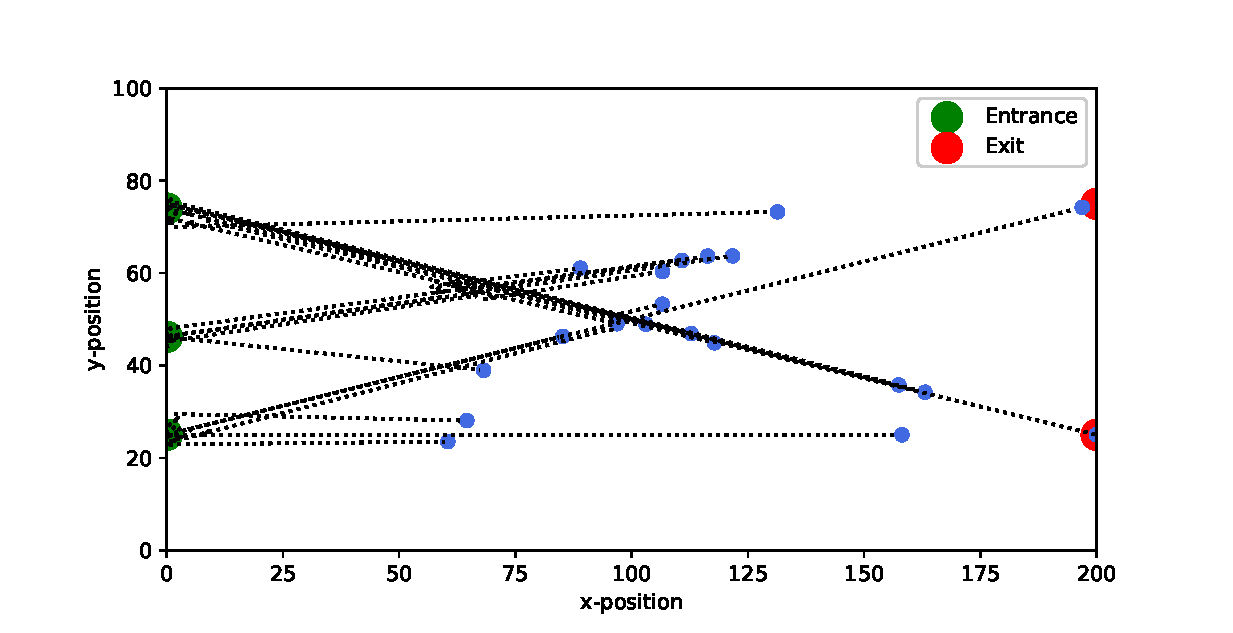
\includegraphics[width=\textwidth]{sample_model_run.eps}
    \caption{Sample model run.}
    \label{fig:sample_model_run}
\end{figure}

\section{Experimental Setup}\label{sec:method:experiments}

With the above model in mind, a simple preliminary experiment was designed to
demonstrate that the Ensemble Kalman Filter method of data assimilation can be
applied to improve the model estimates of agent position of the agent based
model.
In order to achieve this, a class is developed in Python to represent the
Ensemble Kalman Filter.
The Python class representing the model is passed to the filter class as an
argument, along with the filter ensemble size, the frequency with which the
filter should assimilate data, and parameters governing the observational noise.
Upon construction, an instance of the filter class creates an instance of the
model, referred to as the \texttt{base\_model}.
Subsequently, an ensemble of models is created by taking deep-copies of the
\texttt{base\_model}, thus ensuring that each of the ensemble members starts
with model- and agent-attributes that match those in the \texttt{base\_model}.

The instance of the filter class steps forward through time according to the
predict-update cycle.
At each predict step, each of the ensemble member models are stepped forward
once, along with the base model; the frequency with which the filter undertakes
the update step is governed by a parameter known as the
\texttt{assimilation\_period}.
Upon reaching the update step of each cycle, the state of each of the ensemble
member models is updated according to equations found in Section
\ref{sec:method:enkf}.
The ground truth for these experiments is taken to be synthetic data generated
by the \texttt{base\_model}; observations are then generated by adding normally
distributed random noise to the ground truth at each assimilation step.

\begin{itemize}
    \item Population size: 20
    \item Ensemble size:
    \item Assimilation period:
    \item Observation error:
\end{itemize}

%\subsection{Different Types of Ensemble Kalman Filter}\label{sec:method:types}

%Talk about the different types of EnKF and the implications for ensemble size
%\citep{keller2018comparing}.

%\begin{itemize}
    %\item Damping: counteract filter divergence
    %\item Localisation: reduce the effect of spurious correlations
    %\item Hybrid EnKF: Covariance matrix is made up of the weighted sum of the
        %usual covariance matrix and a separate static covariance matrix that
        %encodes prior underlying knowledge about the system
    %\item Dual EnKF: Split the state vector into state and parameters. At
        %assimilation: update parameters, recalculate forecast, update state
    %\item Normal Score EnKF: Developed to handle non-Gaussian PDFs in EnKF. At
        %assimilation: transform state, parameters and measurements into
        %Z-scores, perform EnKF update based on transformed values, transform
        %back from Z-scores
    %\item Iterative EnKF
%\end{itemize}
